%Digital Design and Computer Architecture capitulo 4; datasheet atmega
\paragraph{}
Un sistema integrado o embebido es un sistema digital complejo, compuesto principalmente por CPU, memoria, buses y perif\'ericos, entre otros. La conjunción específica del sistema se denomina arquitectura. El conjunto de los elementos del sistema tambi\'en es conocido como SOC (\textit{System On Chip}).
\begin{figure}[h]
    \centering
    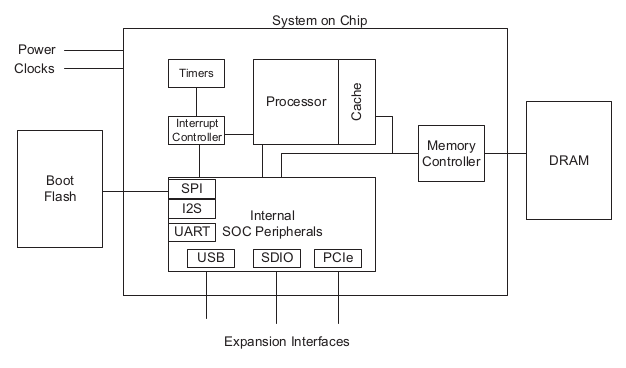
\includegraphics[scale=1, width=.6\textwidth]{soc}
    \caption{Esquema general de un SOC.} 
    \label{fig:soc}
\end{figure}
\paragraph{}
A continuaci\'on se realiza una descripción de los elementos principales que componen el SOC:
\begin{itemize}
\item \textbf{CPU:} Un sistema integrado posee al menos una CPU, la cual se encarga de la ejecuci\'on de los programas, operando con datos e instrucciones. Dependiendo del diseño de la CPU, se tiene una arquitectura de $n$ bits, lo cual implica que el tamaño de los registros y de las direcciones es de $n$ bits. El diseño de la CPU también especifica el uso de un repertorio de instrucciones concreto. Algunos ejemplos de repertorio de instrucciones son ARM, MIPS o CISC. La CPU se consolida como el principal elemento de la arquitectura.
\paragraph{}
   A pesar de que la CPU constituya el elemento principal del sistema integrado, para que todo su procesamiento de datos resulte en trabajo \'util, es necesario el soporte de hardware externo. Dentro de este conjunto de hardware se pueden distinguir:
\item \textbf{Subsistema de memoria:} La memoria en general se encarga de almacenar y servir los datos e instrucciones utilizadas por el procesador. El sistema de memoria se puede descomponer en varios m\'odulos, como por ejemplo: la memoria cach\'e, una memoria f\'isicamente al lado del procesador con una velocidad de trabajo de unos pocos ciclos de procesador; la memoria DRAM, un dispositivo de memoria con un espacio de almacenamiento mayor que la cach\'e, aunque normalmente un orden de magnitud m\'as lenta, u otras memorias externas de diferentes tipos como pueden ser SRAM, FLASH o ROM.
\item \textbf{Controlador de interrupciones:} Este mecanismo gestiona los requerimientos de atención del procesador por parte de los dispositivos, sin necesidad de que este tenga que estar pendiente de la falta de atención continuamente.
\item \textbf{Timers:} El objetivo de estos dispositivos es generar una frecuencia de onda cuadrada estable. Estos dispositivos son imprescindibles para el funcionamiento de la CPU, ya que controlan la frecuencia de trabajo del procesador, o incluso otras tareas como las interrupciones periódicas, programación de eventos o la fecha y hora.
\end{itemize}
\paragraph{Mapa de memoria:} El mapa de memoria es la lista de direcciones accesibles de todos los elementos del sistema: DRAM, controlador de interrupciones... El tamaño total del mapa de memoria dependerá del tipo de arquitectura del procesador y se calcula como $2^n$. Cuando el procesador ejecuta una instrucción de lectura o escritura, la dirección es decodificada por los decodificadores y finalmente enrutada hacia el correspondiente elemento del sistema\footnote{Harris, D. M., & Harris, S. L. (2012). \textit{Digital Design and Computer Architecture} Capítulo 4.}.

\paragraph{AVR Atmega328p:} Como ejemplo de un sistema integrado, se introduce el procesador Atmega328p, el cual he utilizado en el proyecto. 
En las figura \ref{fig:avr-cpu} se muestra un esquema general del sistema integrado Atmega328p. 
\begin{figure}[h]
    \centering
    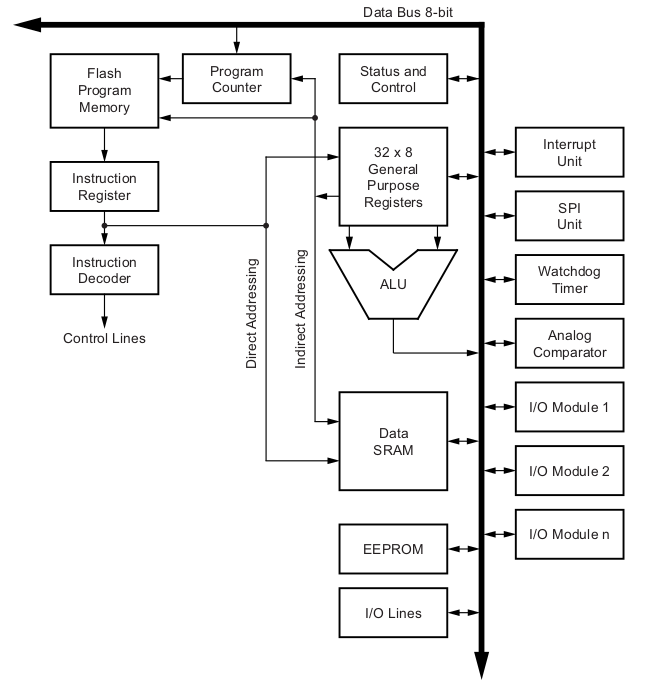
\includegraphics[scale=1, width=.7\textwidth]{avr-cpu}
    \caption{Diagrama de bloques del Atmega328p, en detalle la CPU}
    \label{fig:avr-cpu}
\end{figure}
El Atmega328p es un sistema integrado tipo RISC con un procesador de 8 bit, el cual es capaz de ejecutar una instrucci\'on por ciclo. Esto es posible gracias al diseño de una arquitectura tipo harvard, la cual se caracteriza por disponer de memorias separadas para datos y para las instrucciones del programa. Las instrucciones son ejecutadas con un nivel de segmentaci\'on, lo que permite que, mientras una instrucción está siendo ejecutada, la siguiente instrucción está siendo buscada en la memoria de programa. Es necesario aclarar que la CPU es capaz de trabajar con registros dobles, siendo capaz de direccionar un total de $2^{16}$ posiciones de memoria.
\paragraph{}
Como se puede apreciar en la figura \ref{fig:avr-cpu}, el bloque \textit{Flash program memory} (memoria flash) se corresponde con el espacio de almacenamiento donde se encuentran las instrucciones de nuestro software. Seguidamente se encuentra \textit{Instruction register}, que permite el nivel de segmentaci\'on de las instrucciones. Continuando el esquema, La instrucci\'on a ejecutar es decodificada siguiendo el mapa de memoria y correctamente enrutada al dispositivo correspondiente mediante \textit{Instruction decoder}.
\paragraph{}
Una vez la instrucci\'on es decodificada, pasa a ser ejecutada, entrando en escena la parte de datos. El bloque de los registros, \textit{General purpose Registers} sirven de operandos y junto al bloque \textit{ALU}, se encargan de realizar las operaciones que se requieran. Una vez generados los datos, se vuelcan en el bus de datos y ser\'an recogidos por el dispositivo interesado, gobernados por \textit{Control Lines}. La lectura de los operandos, la operaci\'on con la \textit{ALU} y la escritura del resultado en el banco de registros, se realiza en un solo ciclo de reloj. El \textit{Status Register} es un registro que se actualiza en cada operaci\'on aritm\'etica con las particularidades de dicha operaci\'on: bit $zero$, $carry$, $overflow$, incluso la habilitaci\'on de las interrupciones globales.
\paragraph{}
Como se ha comentado, existen dos mapas de memoria bien diferenciados: instrucciones y datos. La memoria de instrucciones es la flash, la cual tiene una capacidad de $2^{15} \unit{\byte} \approx \SI{32}{\kilo\byte}$, por lo que todas las direcciones de memoria est\'an dedicadas a este elemento.
Por otro lado, se tiene el mapa de memoria de datos, estructurado de la forma mostrada en la figura \ref{fig:mem_datos}.
\begin{figure}[h]
    \centering
    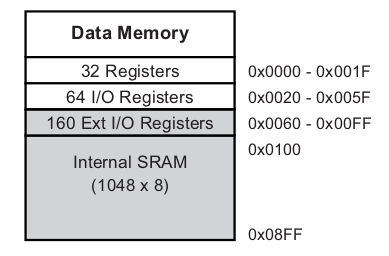
\includegraphics[scale=1, width=.3\textwidth]{avr_datos}
    \caption{Mapa de memoria de datos direccionada por bytes}
    \label{fig:mem_datos}
\end{figure}
Se puede observar en la figura \ref{fig:mem_datos} que el mapa de memoria de datos est\'a separado en distintas regiones: para el banco de registros, para los dispositivos de entrada salida y para la \textit{SRAM}. La \textit{SRAM} es la memoria f\'isica de datos y posee una capacidad de \SI{2}{\kilo\byte}. Al igual que la \textit{FLASH}, esta memoria es accedida mediante registros dobles. El soporte para lidiar con datos de 16 bits se realiza por medio de unos registros especiales, nombrados como X, Y y Z\footnote{Atmel. (n.d.). \textit{ATmega328P Automotive Microcontrollers Datasheet} (Atmel-7810). Recuperado de \url{https://www.microchip.com/wwwproducts/en/ATmega328P}.}.
